\documentclass{article}
\usepackage[fontset=adobe]{ctex}
\usepackage[a4paper, total={6in, 10in}]{geometry}

\title{LSM-KV 项目报告}
\author{廖承凡 522031910632}
\date{2024年 5月 10日}

\usepackage{natbib}
\usepackage{graphicx}
\usepackage{enumitem}
\usepackage{booktabs}
\usepackage{float}
\bibliographystyle{plain}

\begin{document}

\maketitle

\section{背景介绍}

LSMTree(Log-Structured Merge-Tree)是一种用于构建高效的键值存储系统的数据结构。基于LSMTree的键值存储系统通常用于需要高吞吐量和低延迟的应用场景,如分布式数据库、搜索引擎和分布式日志存储系统等。

LSMTree的主要思想是将数据写入多个不同的存储层,然后周期性地合并这些层以维护数据的有序性和一致性。在本项目中,所实现的LSMTree包括以下几个存储层:

\begin{enumerate}
    \item \textbf{MemTable内存表}:是插入数据首先写入的地方,在内存中整理插入内容,便于后面转换为SSTable并存入持久化介质。
    \item \textbf{SSTable键表缓存}:为了加速查找,在本项目中选择将前几层的键表缓存在内存中,这样在查找的时候可以直接从内存里读取而不需要读磁盘,从而实现加速的目的。
    \item \textbf{SSTable键表}:由MemTable转换而来,当MemTable键值对数量超过一定的值时(16KB),便转换为SSTable格式(存储键及其值所在的位置)存入持久化介质。
    \item \textbf{vLog值表}:由于键值对的值的长度并不固定,在本项目中采用键值分离的办法,将所有的值存储在一个vLog文件中,其偏移量保存在SSTable中。
\end{enumerate}

\section{测试}

此部分将展现LSMTree项目的测试,主要分为下面的几个子部分。

\subsection{性能测试}

\subsubsection{预期结果}

\textbf{对常规操作的分析}:对于给出的4种操作,\textbf{插入}(除了发生Compaction的那一次)理论上是耗时最短的,因为它只需要在内存里进行操作,将数据插入到跳表里面。而\textbf{查询}操作次之,如果缓存命中率高(即查询的数据大多是近期插入的),那么也只需要在内存中完成,这样的效率是很高的。但是如果缓存均未命中,则需要进入内存中查找,这样的话就需要磁盘读写等操作,效率就会变得比较低。对于\textbf{删除}操作,需要先进行一次查找,然后如果找到了就插入一个删除标记,因此,它所花费的时间大体上不超过前面两种操作的开销之和。对于\textbf{扫描}操作,应该是花费时间最长的操作,因为它需要暴力搜索每一层出现的键值对,这样才能保证不漏掉任何一个元素。

\subsubsection{常规分析}

首先说明一下在本次常规测试中生成数据的情况:

\begin{enumerate}
    \item 所有的键(类型为uint64\_t)由C++中rand()函数随机生成,范围即是从0到RAND\_MAX (2147483647)。这里说的生成方式在4种操作中均使用(包括get和del,这意味着可能会有很多次查询或删除到不存在的元素,这将导致搜索所有层)。
    \item 所有的值是一个随机长度的字符串,长度范围1到1000随机,同时字符取自10个阿拉伯数字和52个大小写字母。
\end{enumerate}

在常规分析中,首先对操作的延迟进行测试,在本项目中,分别对操作数据量为1e4, 1e5, 1e6的四种操作进行了测试,三种数据量下的平均测试结果如下表所示:

\begin{table}[h]
    \centering
    \begin{tabular}{ccccc}
        \toprule
        测试数据量 & Put       & Get       & Scan          & Delete     \\
        \midrule
        1e4        & 15561.9ns & 613.593ns & 4.96419e+07ns & 689.88ns   \\
        1e5        & 19434.2ns & 17345.4ns & 4.62088e+08ns & 16905.7ns  \\
        1e6        & 21917.7ns & 125992ns  & 4.44253e+09ns & 121412ns   \\
        平均值     & 18971.3ns & 47983.7ns & 1.65142e+09ns & 46335.86ns \\
        \bottomrule
    \end{tabular}
\end{table}

由于测试数据大小对层数影响很大,而层数也会在较大程度上影响三种操作的效率,因此上面的性能差异其实是比较大的。但是既然要测试不同数据,那这样的差异便是我们预期之内的。不过我们也可以发现,数据量大小为1e4的时候Get和Del操作非常快,这是因为在数据量较小的时候,有较大比例的SSTable是保存在缓存中的,而缓存的查询速度比磁盘要快很多。

而对于四种操作的吞吐量,在平均意义上,只需要对时延取倒数即可。因此,由上面的表,我们得到下面的平均吞吐表:

\begin{table}[h]
    \centering
    \begin{tabular}{ccccc}
        \toprule
        操作名称   & Put   & Get   & Scan  & Delete \\
        \midrule
        平均吞吐量 & 52711 & 20840 & 0.606 & 21582  \\
        \bottomrule
    \end{tabular}
\end{table}

\subsubsection{索引缓存与Bloom Filter的效果测试}

针对给出的三种缓存模式测试,根据我代码实现的方式,分别采用如下的方法测试:

\begin{enumerate}
    \item 内存中没有缓存SSTable的任何信息,从磁盘中访问SSTable的索引,在找到offset之后读取数据:去除代码中在每一层实现的二分搜索,改为顺序搜索,同时将SSTable缓存层数设置为0,相当于并不知道SSTable的信息,仅仅从磁盘里获取信息。
    \item 内存中只缓存了SSTable的索引信息,通过二分查找从SSTable的索引中找到offset,并在磁盘中读取对应的值:最终的代码中已经实现索引的缓存,这里只需要将SSTable缓存层数设置为0即可。
    \item 内存中缓存SSTable的Bloom Filter和索引,先通过Bloom Filter判断一个键值是否可能在一个SSTable中,如果存在再利用二分查找,否则直接查看下一个SSTable的索引:最终的代码即是这样实现的。
\end{enumerate}

在本次测试中,键值对的数量为1e5,而值的选取方式和前面的相同。据此,测试结果如下表:

\begin{table}[H]
    \centering
    \begin{tabular}{cc}
        \toprule
        测试序号 & Get平均时延 \\
        \midrule
        1        & 789367ns    \\
        2        & 21266.3ns   \\
        3        & 18124.3ns   \\
        \bottomrule
    \end{tabular}
\end{table}

从上面的表里可以看出,在内存中缓存SSTable的索引可以极大地降低GET操作的时延,因为缓存索引不仅可以使得查找时不需要读文件就可以找到对应的那一些SSTable,还可以进行二分搜索。而进一步再缓存一些SSTable也有效率的提升,但是提升就没有那么明显了,因为在我们可以通过索引信息快速定位到对应的SSTable,然后从磁盘中读出该文件,查询得到offset后进一步进入vLog中进行查找。而缓存BloomFilte的话,可以快速判断该键值对是否存在于该SSTable中,于是最多只会比仅仅缓存索引信息的情况少读写总层数数量的文件。但是缓存每一个SSTable的BloomFilter是一件很耗内存的事情,因此需要权衡好这一个trade off。

\subsubsection{Compaction的影响}

在给定一定的时间间隔,不断插入数据的情况下,通过子进程计时、父进程计数的方式,得到了每一段时间内Put操作的吞吐量如下表:

\begin{figure}[h]
    \centering
    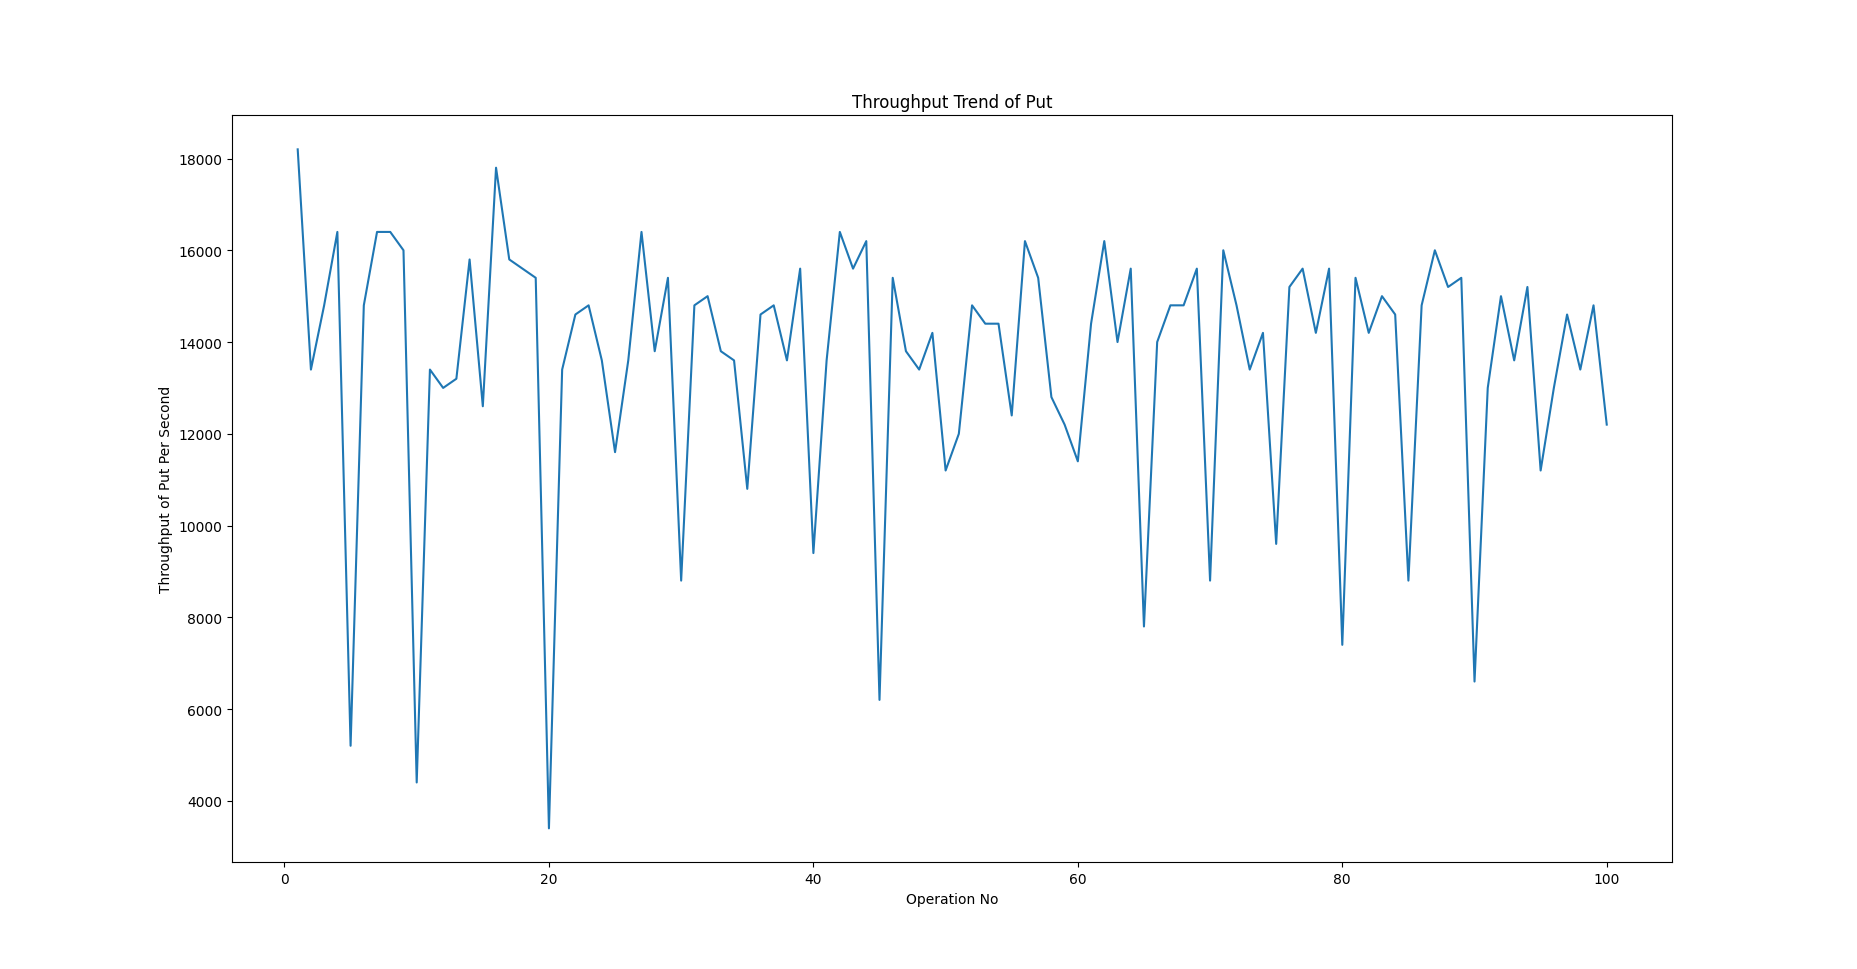
\includegraphics[width=0.8\textwidth]{images/compaction.png}
    \caption{LSMTree的Put操作吞吐量的变化趋势}
    \label{compaction}
\end{figure}

需要说明的是,由于本项目中的LSMTree开启编译优化最快速度(-Ofast)后,运行速度是比较快的,因此此处如果选择测量每秒的操作数量,绘制出的图会非常不显著。因此,本测试里使用的时间间隔是5e3us(即5毫秒),然后经过换算得到真正的吞吐量。另外,在这个测试里,由于是给定时间测量操作的数量,因此并没有去除掉生成数据的时间(由随机数生成键其实可以忽略不计,但是生成值需要随机生成至多1000个字符),导致吞吐量基本在14000左右,比第一节常规测试中的吞吐量要低一点。

从图中可以看出,有几个很明显的吞吐量降低的点,这就意味着在这个时间段内发生了compaction,这导致了它存储效率的突然降低。但是降低的幅度也均有不同,这可能是由于compaction合并的层数不相同导致的。因为compaction是一个递归操作,如果某一层的compaction完成导致下一层的文件数量超出了限制,那么又要继续进行compaction,从而导致时间变得更长,吞吐量降低。

\subsubsection{Bloom Filter 大小配置的影响}

在我的代码实现中,BloomFilter的大小定义在了一个头文件里面,其他的存储结构的数量也都是根据这些变量计算出来的,因此只需要对这个变量进行修改就可以达到测试的目的。在这个测试中,我采取的Get和Put的数量均为1e5次,键值对的生成方式依然和前面提到的一样。通过对1KB至12KB的过滤器大小进行测试,得到数据后绘制出下面的图:

\begin{figure}[h]
    \centering
    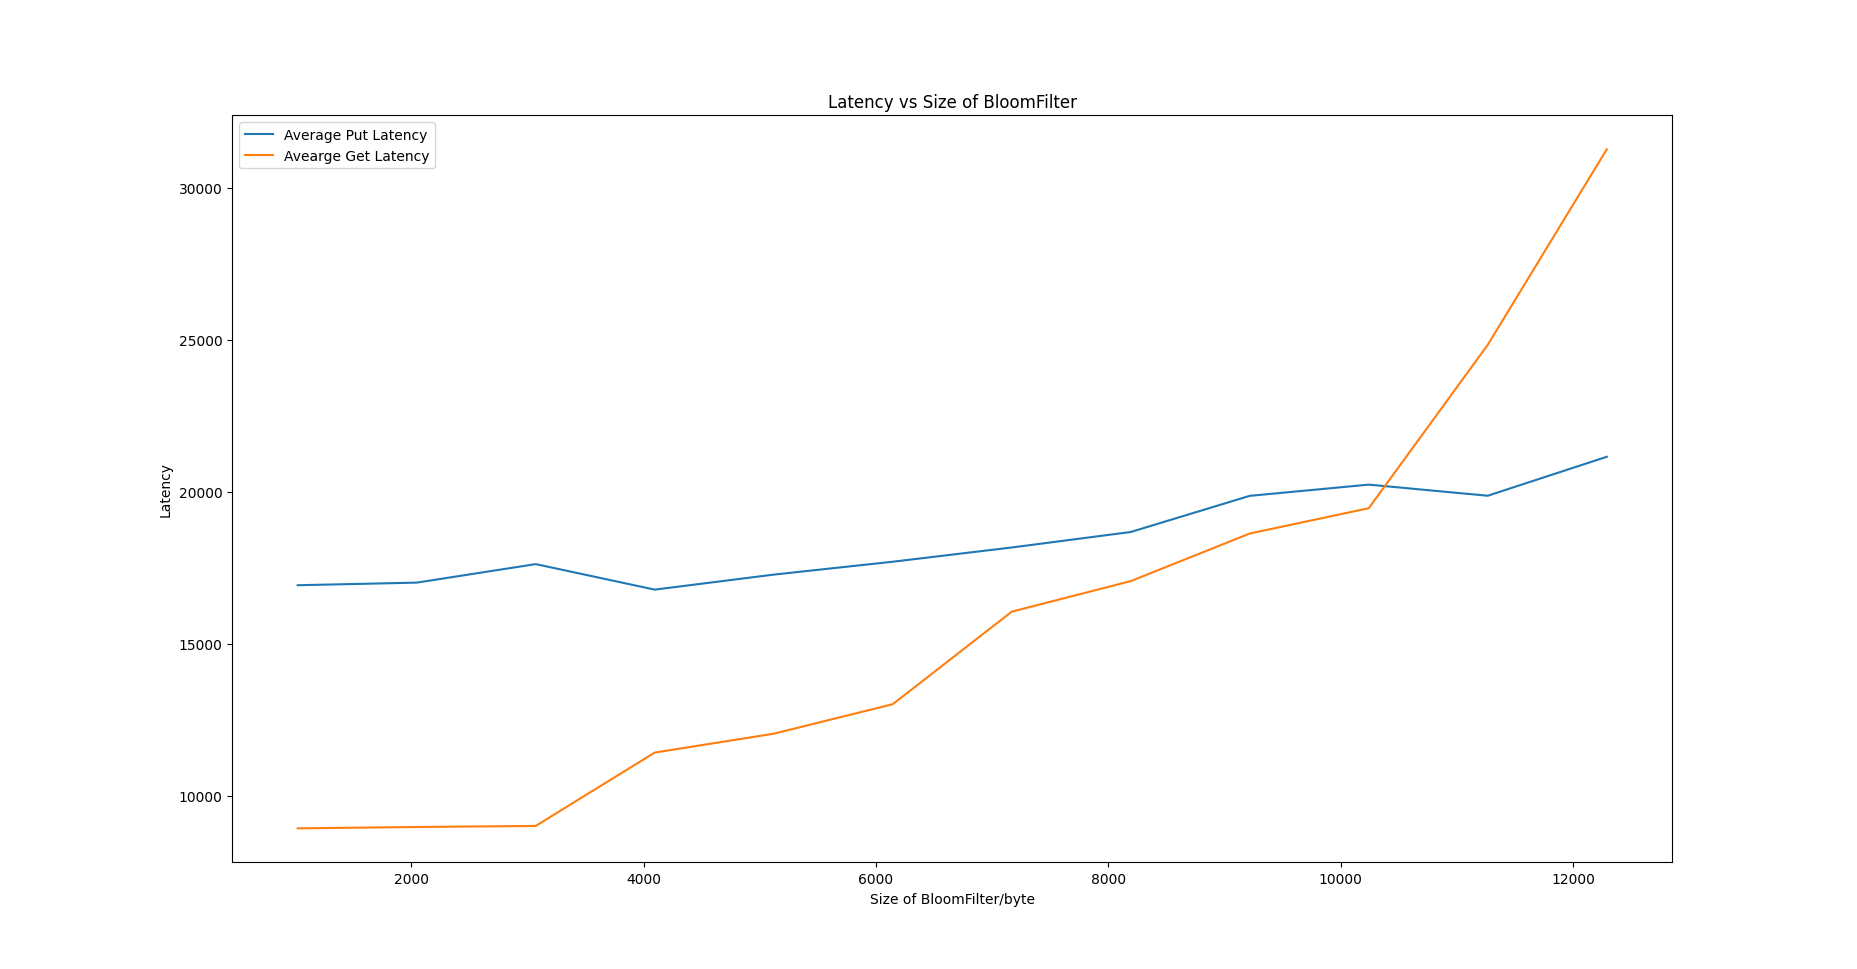
\includegraphics[width=0.8\textwidth]{images/filter.png}
    \caption{不同大小的布隆过滤器下操作的时延}
    \label{filter}
\end{figure}

很反直觉的一点是,在上面的图里,时延几乎是一直在递增的,这就需要从我的代码结构来解释了。事实上,在我的代码里,为了节省空间,布隆过滤器的存储是以bit为单位的。这就意味着,即使它的大小只有1024个字节,我也可以存储8096个代表元素是否存在的哈希值。而布隆过滤器即使是只有1024个字节,里面存储的SSTable Entry也只有638个,由于每个Entry会计算4次哈希值(在我的代码实现中),假如完全不冲突,最多将占据2552个比特,不到1/3,因此才会出现上面的情况。

但是由于数据具有随机性,上面的数据是多次测试取了大致的平均值得出的,但是在测试的过程中发现时延还是具有较高的随机性。这必然与系统的CPU调度等存在一定关系,但是总体上的趋势是稳定的。

总之,如果希望LSMTree的性能可以达到最高,可能需要继续进行多次测试,找到最适合的布隆过滤器的大小。

\section{结论}

总体来说,这一个Project是相当具有挑战性的。我花了很多的时间在设计、编码、重构这个项目,一步一步对整个数据结构进行优化。在优化的过程中,也可以体会到数据结构中很多小trick的作用,比如分层、二分、缓存等等,在这个项目中都起到了很大的作用。

最后在开启编译器加速最大速度的情况下,可以在40s左右完成给定的正确性测试,对这个结果我是比较满意的。

另外,由于在编写代码的过程中,我也很注意代码结构,将很多用到的常量、结构等都写在一个头文件definition.h中,因此在测试的时候基本上只需要更改这一个头文件里的配置即可,最后得到的结论也比较不错。总之,这个项目极大地锻炼了我的代码能力,也让我领会到了数据结构的巧妙。

\section{致谢}

其实整个项目的结构基本上都是我自己思考、重构出来的,但是也很感谢身边同学愿意与我一起进行项目的讨论,一起研究C++的一些小trick。

另外,我也从CSDN论坛上获得了一些启发,比如在对SSTable不同层的文件进行命名的时候,虽然运行测试都没出现过问题,但是可以很容易想到一些情况下,文件会有一定概率重名,这样就会导致对文件的覆盖写。而在查阅了CSDN的一篇帖子中提到的方法后,我最终采用了时间戳+进程号+文件ID的方式进行命名,这样可以保证一定不会出现问题。


\section{其他和建议}

Debug真的很困难!最开始写这个项目的时候,先写了只有一层的LSMTree,在修正了很多的bug之后,终于是正确通过了正确性测试。但是!在后面写分层的时候发现出现了文件覆盖写问题,而这个问题在前面只有一层的LSMTree中也会出现!但是它当时通过了正确性测试!!!

于是后面就出现了很多,在后一个版本修改前一个版本的错误的情况。

以及,我是把第一次作业中写的跳表拿过来直接用的,但是后面检查出我那时的跳表实现有bug!不过是因为第一次作业的时候并没有用到那一个成员函数,只是当时觉得应该写上就写在了代码里面,但是这个函数是有错误的。。。

总之虽然道路艰辛,但是这个Project的质量比前两个Lab要高太多了(笑)。

\end{document}
